\usetikzlibrary{decorations.markings}
\tikzset{-dot-/.style={decoration={
  markings,
  mark=at position #1 with {\fill circle (2pt);}},postaction={decorate}}}

\begin{subfigure}{0.3\textwidth}
\centering
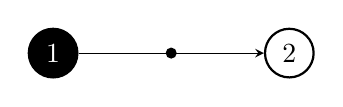
\begin{tikzpicture}[node distance={30mm}, main/.style = {draw, circle, thick}, fired/.style = {draw, circle, thick, fill=black, text=white}]
\node[fired] (1) {$1$};
\node[main] (2) [right of=1] {$2$};
\draw[->, >=stealth, -dot-=0.5] (1) -- (2);
\end{tikzpicture}
\caption{}
\end{subfigure}

\begin{subfigure}{0.3\textwidth}
\centering
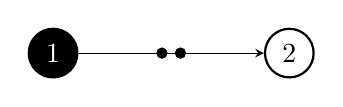
\begin{tikzpicture}[node distance={30mm}, main/.style = {draw, circle, thick}, fired/.style = {draw, circle, thick, fill=black, text=white}]
\node[fired] (1) {$1$};
\node[main] (2) [right of=1] {$2$};
\draw[->, >=stealth, -dot-=0.55, -dot-=0.45] (1) -- (2);
\end{tikzpicture}
\caption{}
\end{subfigure}

\begin{subfigure}{0.3\textwidth}
\centering
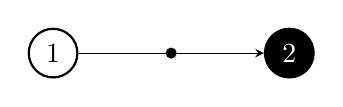
\begin{tikzpicture}[node distance={30mm}, main/.style = {draw, circle, thick}, fired/.style = {draw, circle, thick, fill=black, text=white}]
\node[main] (1) {$1$};
\node[fired] (2) [right of=1] {$2$};
\draw[->, >=stealth, -dot-=0.5] (1) -- (2);
\end{tikzpicture}
\caption{}
\end{subfigure}

\begin{subfigure}{0.3\textwidth}
\centering
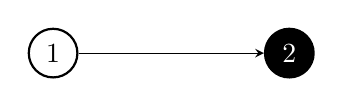
\begin{tikzpicture}[node distance={30mm}, main/.style = {draw, circle, thick}, fired/.style = {draw, circle, thick, fill=black, text=white}]
\node[main] (1) {$1$};
\node[fired] (2) [right of=1] {$2$};
\draw[->, >=stealth] (1) -- (2);
\end{tikzpicture}
\caption{}
\end{subfigure}

% \begin{subfigure}{0.34\textwidth}
% \centering
% \begin{tikzpicture}[node distance={30mm}, main/.style = {draw, circle, thick}, fired/.style = {draw, circle, thick, fill=black, text=white}]
% \node[fired] (1) {$1$};
% \node[main] (2) [right of=1] {$2$};
% \draw[->, >=stealth, -dot-=0.5, -dot-=0.1] (1) -- (2);
% \end{tikzpicture}
% \caption{}
% \end{subfigure}
